	\thispagestyle{empty}
	
	\begin {center}
	\begin{tabular} {|p {3cm}|p{8cm}|p{4.55cm}|}
	 \hline 
	\vspace{1mm}
	 \centering{
\includegraphics[width=0.20\textwidth,page=1]{Alle/TGM_logo.pdf}} &
	\centering{\normalsize{\textbf{HTBLVA Wien 20}}\par\small{\textbf{H�here Technische Lehranstalt f�r}\par Biomedizin- und Gesundheitstechnik}} &
		\small{\bfseries{Reife- und\par Diplompr�fung}}\\ 
		\hline
	\end{tabular}
	
	\vspace{5mm}
	\Large{\textbf{DIPLOMARBEIT\\}}
	\vspace{1mm}
	\small{\textbf{DOKUMENTATION\\}}
	\vspace{5mm}  
	
		\begin{tabular} {|p {5.7cm}|p{10.3cm}|}
		 \hline 
			\bfseries{\small{Namen der\par Verfasser/innen}} & \small{Fatiha Banata, Claudia Fuchs, Julia Gartner, Sumaiya Hossain}\\
		 \hline
		  \bfseries{\small{Jahrgang\par Schuljahr}} & \small{5AHBG 2022/23}\\
		 \hline 
		  \bfseries{\small{Thema der Diplomarbeit}} & \small{Sleep-Analyzer}\\ 
		 \hline 
		  \bfseries{\small{Kooperationspartner}} & \small{/}\\ 
		 \hline
		\multicolumn{2}{l}{\large{ \textbf{}}}\\
		 \hline
		  \bfseries{\small{Aufgabenstellung}} & \small{Im Rahmen einer Machbarkeitsstudie soll der Schlaf eines Anwenders durch Messung von Biosignalen analysiert werden. Dazu sollen verschiedene Messmethoden entwickelt und auf ihre Tauglichkeit getestet werden. Die gemessenen Daten sollen anschlie�end in einer Datenbank verwaltet und f"ur den Anwender in einer App dargestellt werden.}\\
		 \hline
		\multicolumn{2}{l}{\large{ \textbf{}}}\\ 
		 \hline
		  \bfseries{\small{Realisierung}} & \small{Die REM-Schlafphase wird mittels Elektrookulogramm zur Messung von Augenbewegungen detektiert und die vom ESP8266 gemessenen Daten werden "uber WLAN an eine Datenbank weitergegeben. Die Ausgabe der Daten erfolgt "uber ein App-Interface. }\\   
		 \hline
		\multicolumn{2}{l}{\large{ \textbf{}}}\\ 
		 \hline
		  \bfseries{\small{Ergebnisse}} & \small{Augenbewegungen lassen sich mittels EOG-Schaltung messen und die Daten, durch ein RTC-Modul mit einem Zeitstempel versehen, an die Datenbank schicken. In der App k"onnen die Daten f"ur den Anwender angezeigt werden.}\\
		 \hline
		\end{tabular}
	\end {center}
\thispagestyle{empty}
		
\newpage
\thispagestyle{empty}

	\begin{centering}
	\begin{tabular} {|p {3cm}|p{8cm}|p{4.55cm}|}
	 \hline 
	\vspace{1mm}
	 \centering{
\includegraphics[width=0.20\textwidth,page=1]{Alle/TGM_logo.pdf}} &
	\centering{\normalsize{\textbf{HTBLVA Wien 20}}\par\small{\textbf{H�here Technische Lehranstalt f�r}\par Biomedizin- und Gesundheitstechnik}} &
		\small{\bfseries{Reife- und\par Diplompr�fung}}\\ 
		\hline
		\multicolumn{3}{l}{\large{ \textbf{}}}\\
	\end{tabular} 
	
   \vspace {1mm}
	
		\begin{tabular} {|p {5.7cm}|p{10.3cm}|}
		 \hline 
			\bfseries{\small{Typische Grafik, Foto etc.\par (mit Erl�uterung)}} & \vspace{0.0mm} \small{
			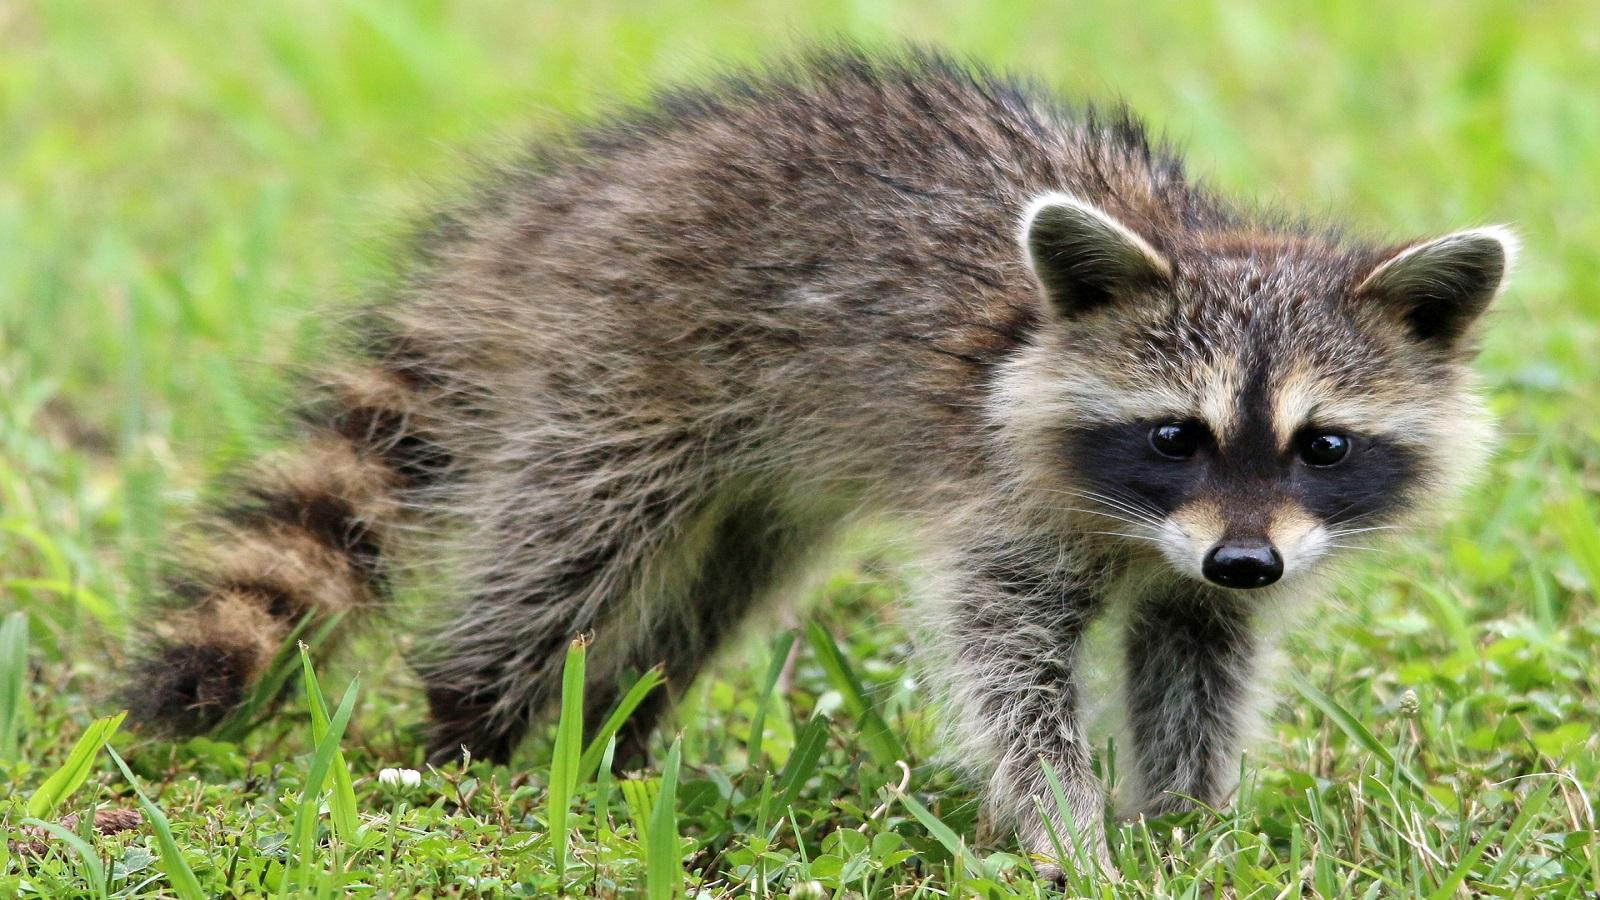
\includegraphics[width=0.666\textwidth]{Alle/Bild.jpg} \par BILDBESCHREIBUNG
			}\\
		 \hline
		  \multicolumn{2}{l}{\large{ \textbf{}}}\\
		 \hline
		  \bfseries{\small{Teilnahme an Wettbewerben,\par Auszeichnungen}} & \small{/}\\
		 \hline 
		  \multicolumn{2}{l}{\large{ \textbf{}}}\\
		 \hline
		  \bfseries{\small{M�glichkeiten der\par Einsichtnahme in die Arbeit}} & \small{Abteilungsadministration}\\ 
		 \hline 
		  \multicolumn{2}{l}{\large{ \textbf{}}}\\
		\end{tabular} %done 
		
		\begin{tabular} {|p {5.7cm}|p{5.3cm}|p{4.6cm}|}
		 \hline
	   \vspace{5mm}
		  \bfseries{\small{Approbation\par (Datum/Unterschrift)}} \vspace{5mm} & \tiny{Pr�fer/Pr�fernin} & \tiny{Direktor/Direktorin\par Abteilungsvorstand/Abteilungsvorst�ndin}\\ 
		 \hline 
		\end{tabular} 
		\end{centering}
		
\thispagestyle{empty}

